\section{Entropy and Mutual Information}

\textbf{Entropy} -- quantifies information content of a random variable. It is
generally measured in bits and can be though of as the expected information
content when we sample a random variable once. Entropy for a discrete random
variable is defined in \autoref{eq:entropy}.

\begin{equation}
  H(X)=-\sum _{i=1}^{n}{P (x_{i})\log P(x_{i})}
\label{eq:entropy}
\end{equation}

Consider a random variable $X$ s.t $P(X=1) = P(X=0) = 0.5$, this tells
us that $H(X) = 1$ and every time we sample $X$ we are expected to gain 1 bit of
information.

Similarly for a random variable $Y$ s.t $P(X=0) = 0.5, P(X=1) = P(X=2) = 0.25$,
we have $H(Y) = 1.5$

\textbf{Conditional Entropy} -- quantifies the amount of information needed to
describe an outcome of variable $Y$ given that value of another random variable
$X$ is already known. Entropy of $Y$ given $X$ is written as $H(Y|X)$.
Conditional Entropy for a discrete random variable is defined in
\autoref{eq:condEntropy}

\begin{equation}
H(Y|X)\ =-\sum _{x\in {X},y\in {Y}}p(x,y)\log {\frac {p(x,y)}{p(x)}}
\label{eq:condEntropy}
\end{equation}

Consider a random variable pair $X$ and $Y$ s.t 
$$P(X=0,Y=0) = P(X=0,Y=1) = 0.25, P(X=1,Y=0) = 0.5, P(X=1,Y=1) = 0$$
then $H(Y|X) = 0.5$ and $H(X|Y) \approx 0.6887$, while $H(X) = 1$ and $H(Y)
\approx 0.8112$

\textbf{Mutual Information (MI)} -- is a measure between two random variables,
it builds on top of entropy and measures how much information the variables have
in common. It quantifies information gained about one variables when observing
the other. Mutual information is generally computed either explicitly using the
probabilities as in \autoref{eq:miExplicit} or using entropies as in
\autoref{eq:miEntropy}.

\begin{equation}
      I(X,Y)=\sum _{y\in Y}\sum _{x\in X}{p(x,y)\log {\left({\frac
      {p(x,y)}{p(x)\,p(y)}}\right)}} 
\label{eq:miExplicit}
\end{equation}

\begin{equation}
  I(X, Y) = H(X) - H(X|Y)
\label{eq:miEntropy}
\end{equation}

Consider the random variables $X$ and $Y$ as before in the conditional entropy
section. 
$$P(X=0,Y=0) = P(X=0,Y=1) = 0.25, P(X=1,Y=0) = 0.5$$
Here we can see that $I(X,Y) \approx 0.3113$

\section{Neural Network}

\textbf{Neural Networks} are a machine learning framework that is intended to
solve the problem of prediction or classification of data. 

Suppose we have a dataset:
$$ (x_i, y_i) \text{ for } i = 1,...,N, x_i \in \mathbb{R}^d, y_i \in \mathbb{R}^{d^\prime}$$ 
where $x_i$ is the input to the Neural Network and $y_i$ is the label or the
value we want the neural network to predict. Suppose we are trying to classify
if an image contains a cat or no, then $x_i$ would be an encoding of an image
and the label $y_i$ could be 1 if the image contains a cat and 0 if it does not.

The network is structured in layers where every layer holds an intermediate
representation of the final prediction output, lets call this intermediate
representation an activation of that specific layer. For our purposes we will
define a neural network to be a sequence of functions
$f_{\theta}^1,f_{\theta}^2,... ,f_{\theta}^N$ that are parameterized by weights
$\theta$ s.t

\begin{align*}
  \text{let } t_0 &= x, \\
    t_0 \rightarrow f_{\theta}^1(t_0) &= t_1,\\
    t_1 \rightarrow f_{\theta}^2(t_1) &= t_2,\\
    &...\\
    t_{N-1} \rightarrow f_{\theta}^N(t_{N-1}) &= t_N,\\
    \text{let } y &= t_N
\end{align*}

We have one function for each layer transition of the neural network this allows
us to extract the activation of a specific layer as in \autoref{eq:layerL}, we
will need to get access to intermediate layers in our experiments.

\begin{figure}[H]
  \[ t_l = f_{\theta}^l(f_{\theta}^{l-1}(...(f_{\theta}^1(x)))) \]
  \caption{activation of layer l for input x}
  \label{eq:layerL}
\end{figure}

\textbf{Stochastic Gradient Descent} Each of the transition function are
parameterized by the weights function $\theta$. The $\theta$ function is
directly controlled by Stochastic Gradient Descent (SGD) algorithm.  SGD is an
algorithm for training a neural network it gradually updates the weights
$\theta$ according to some goal such as minimising the prediction error.  SGD is
an iterative process, it has a notion of epochs where one iteration of the
algorithm advances epochs by one, this implies that $\theta$ function depends on
which epoch we are currently at thus it must take the epoch number as an
argument -- $\theta(e)$.

\section{The Information plane}

\subsection{Setup}

The Information plane is a way of visualizing the Neural Networks training
process trough the information domain. By looking at mutual information between
the input $X$ the intermediate neural network layer activations $T$ and the
label $Y$ we can see how the information flows trough the network.

Mutual Information, as we defined it, is only applicable to Probability
distributions, however we currently only have the datset 
$(x_i, y_i) \text{ for } i = 1...N$
, if we assume that every input $x_i$ equally likely we can provide a routine
that defines our probability distribution.

For convenience lets define $F_{\theta}^t$ to be the activation of layer t given
input $x$, i.e
\begin{equation}
  F_{\theta}^t(x) = f_{\theta}^t(f_{\theta}^{t-1}(...(f_{\theta}^1(x))))
  \label{eq:bigF}
\end{equation}


Consider \autoref{fig:rxty}, the routine defines the random variables
$X,T_{e,t},Y$. Here $T_{e,t}$ is the distribution of layer $t$ for the epoch $e$,
$X$ and $Y$ is the original data with assumption that it is uniformly
distributed. 

Using the probability distributions we now have values:
\begin{itemize}
  \item{
      $I(T_{e,t}, X)$ -- Mutual Information between the input distribution and the
      layer activations 
    }
  \item{
      $I(T_{e,t}, Y)$ -- Mutual Information between the label distribution and the
      layer activations.
    }
\end{itemize}
This allows us to generate the Information plane.


\begin{figure}[H]
    \begin{pythonfigure}
      def rxty(e, t):
        pick i ;$\sim$; Uniform {1...N}
        return ;$(x_i, F_{\theta(e)}^t(x_i), y_i)$;
    \end{pythonfigure}
    \caption{Definition of correlated random variables $X, T_{e,t}$ and, $Y$}
    \label{fig:rxty}
\end{figure}

\subsection{Visualization}

The Information plane visualizes the whole training process, in order to
generate the information plane we need $I(X,T_{e,t})$ and $I(Y,T_{e,t})$ for every
epoch $e$ and every layer $t$.

Consider for now that we only trained our neural network for one epoch, the
\autoref{fig:Ip1} shows an example of this. 

In this case the network consists of 5 layers, in the figure every node
corresponds to a distinct layer. The lines between the nodes help us distinguish
epochs from each other and gives helps us to see the order of the layers, the
upper-right-most node corresponds to the first layer in the neural network, the
lower-left-most node corresponds to the fifth and last layer of the network.

\begin{figure}[H]
  \centering
  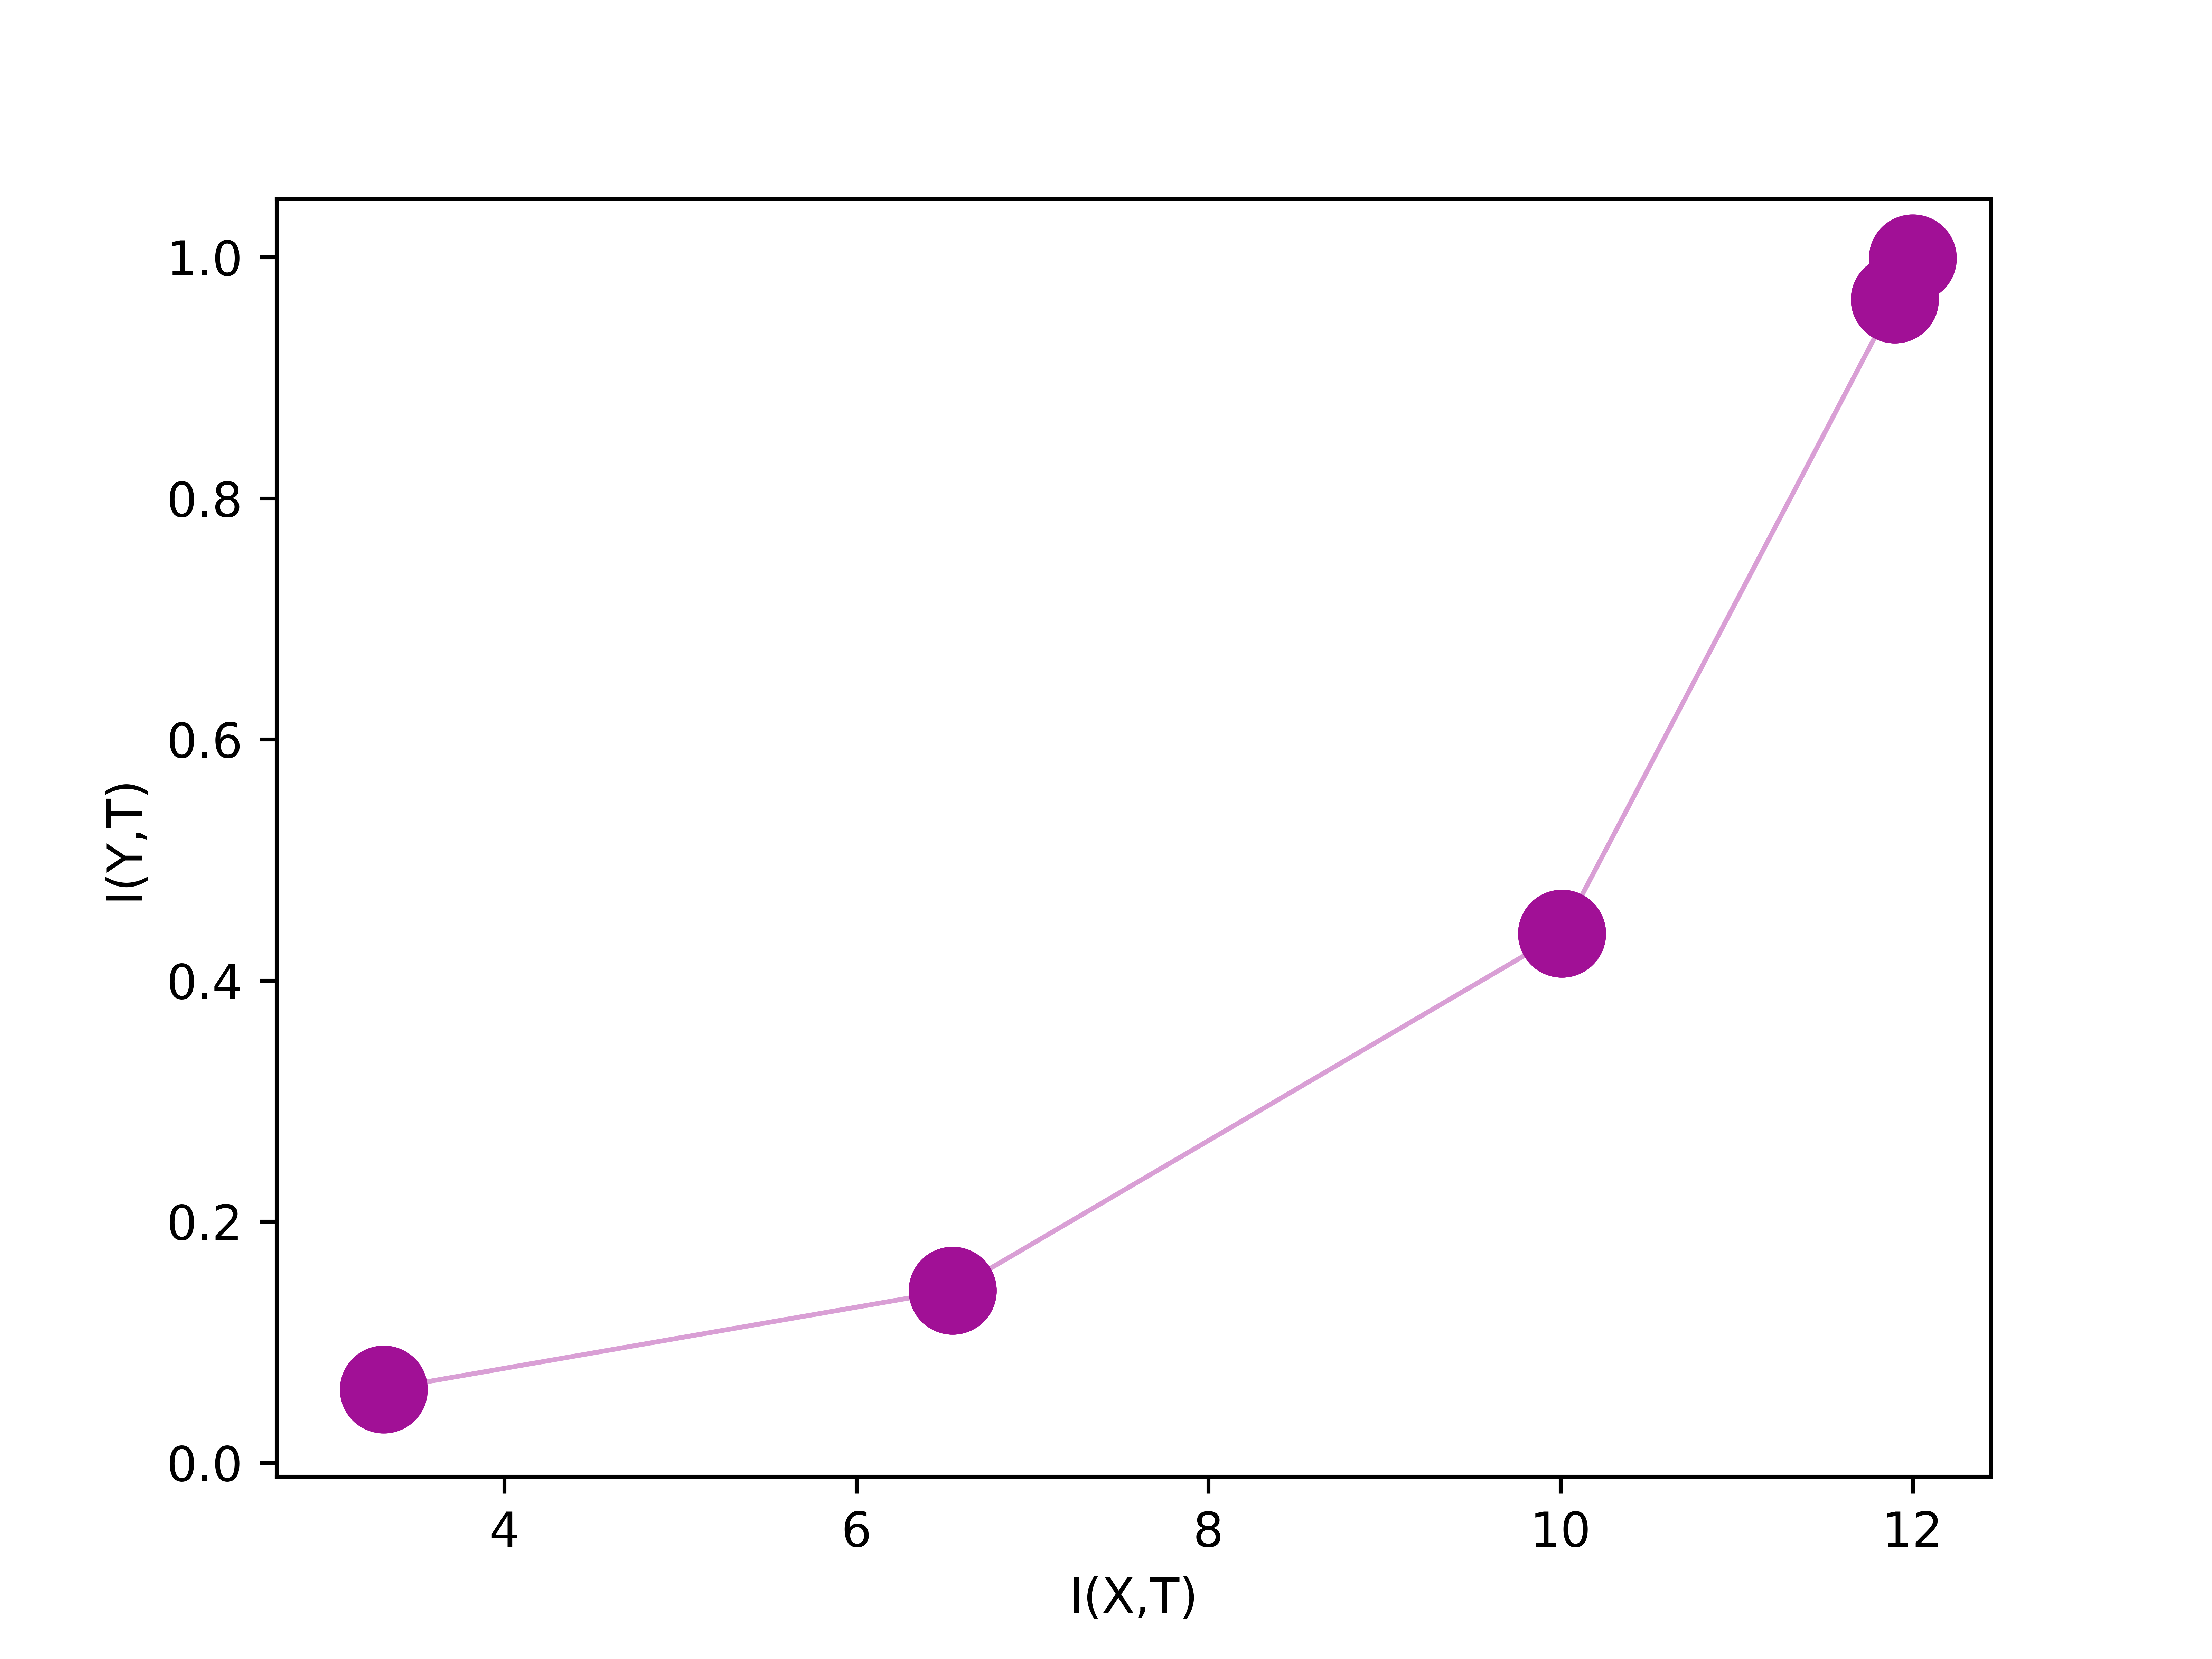
\includegraphics[width=0.60\textwidth]{figs/ip_1v2.png}
  \caption{
    information plane for a neural network with 5 layers, which was only trained
    for one epoch.
  }
  \label{fig:Ip1}
\end{figure}

Consider now \autoref{fig:Ip2}, it shows an information plane for a full
training phase. The color signifies what epoch the data belongs to and let us
see how the network progressed over time. We can see that at the start $I(Y,
T_{1,4}) \approx 0$ meaning the network has not preserved any information about
the label distribution $Y$, but by the end of the training we see $I(Y,
T_{10^4,4}) \approx 1$ which means we have preserved almost all the information
about the label.


\begin{figure}[H]
  \centering
  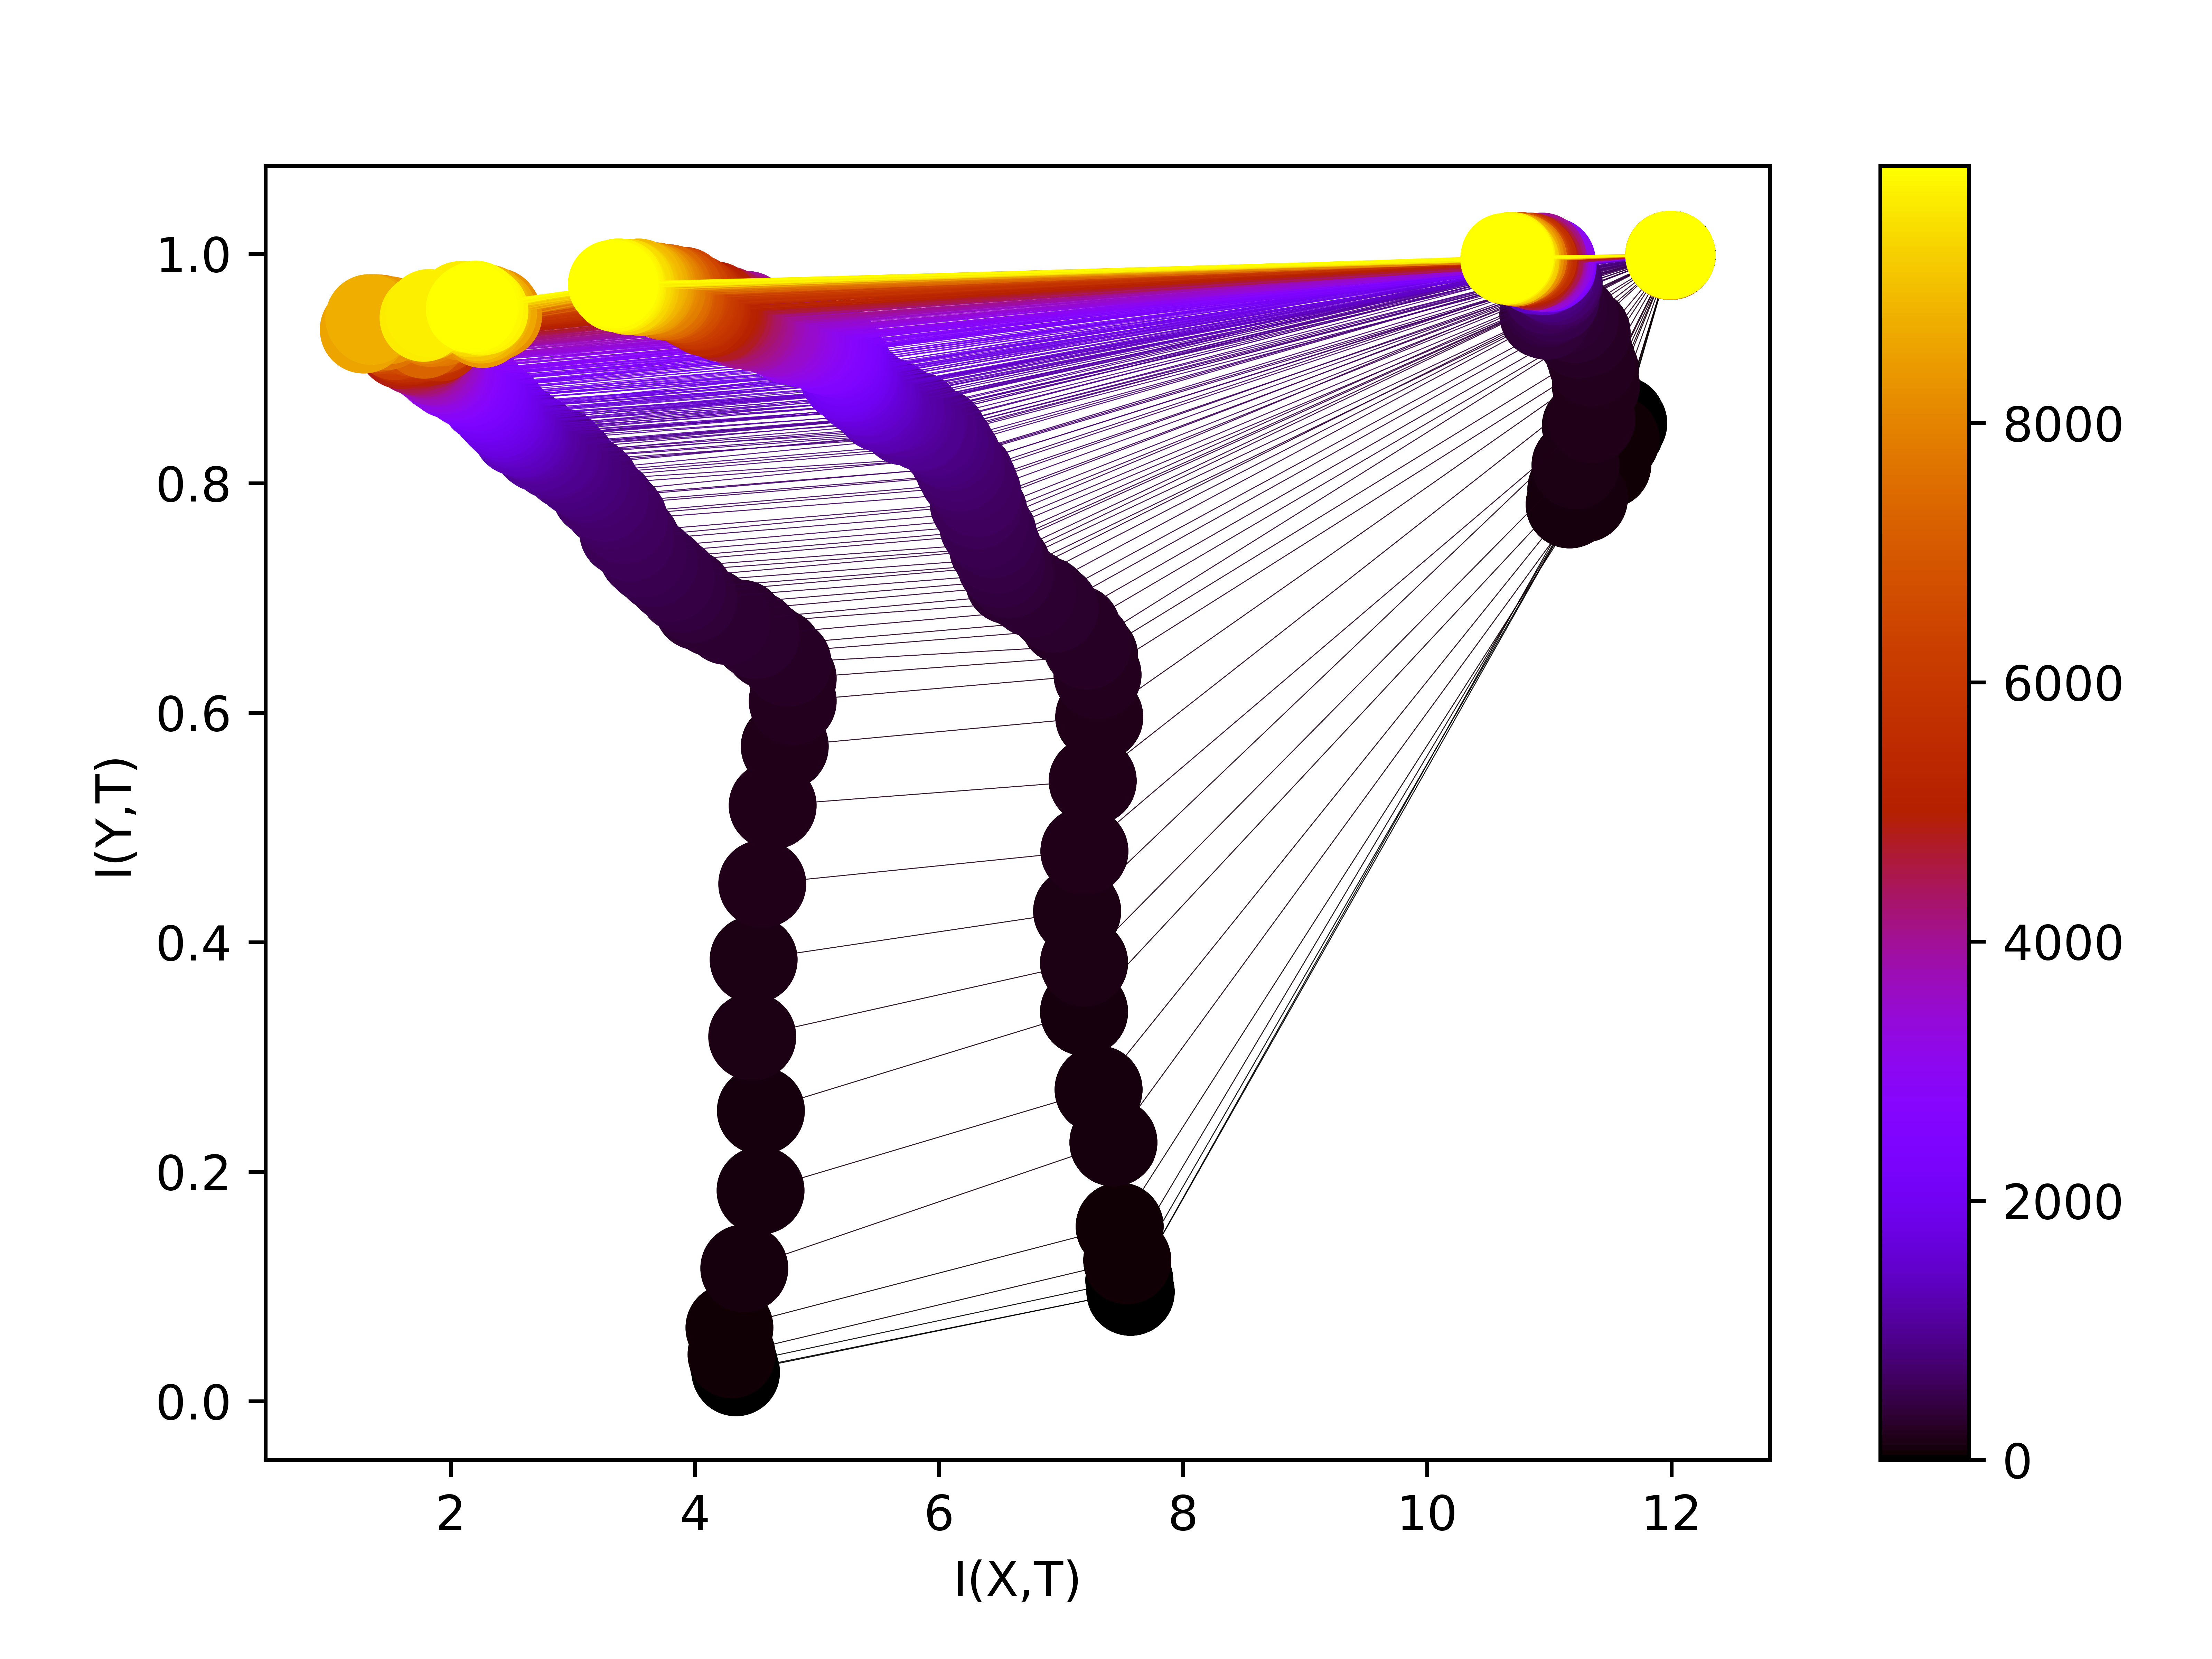
\includegraphics[width=0.60\textwidth]{figs/ip_10000.png}
  \captionof{figure}{
    Information plane for a neural network with 4 layers, which was trained for
    approximately $ 10\,000 $ epochs. The Neural Network was trained on the same
    dataset as used by Tishby, 2017, hence entropy of the input $H(X)$ is 12 and
    entropy of the label $H(Y)$ is 1.
  }
  \label{fig:Ip2}
\end{figure}

\subsection{Interpretation of the Information Plane}

Let us once again consider \autoref{fig:Ip2}, we can see two phases in the figure
Tishby has named them The Fitting Phase and The Compression Phase.

\subparagraph{The Fitting Phase} In \autoref{fig:Ip2} the neural network is in
the fitting phase from the start of the training up until epoch $\sim$1500. The
duration of the fitting phase varies heavily on the training parameters and is
most influenced by the size of our input dataset. The fitting phase is
characterized by:
\begin{itemize}
  \item{
      A rapid increase in $I(Y, T_{e,t})$, the information about the label, as we
      advance trough the epochs $e$, the increase is especially visible in the
      later layers, in our case layers 3 and 4.
    }
  \item{
      Either an increase or no change in $I(X, T_{e,t})$, the information about
      the input, as we advance trough the epochs $e$, in our case we see very
      little change in $I(X,T_{e,t})$.
    }
\end{itemize}

During the fitting phase a neural network tries to memorize the data and make
predictions based on the observations, this means that the network may learn
useless features that only superficially correlate with the correct label.

\subparagraph{The Compression Phase} In \autoref{fig:Ip2} the neural network
enters the compression phase when the fitting phase ends around epoch $\sim$1500
and lasts until we finish the training process. The compression phase is
characterized by:
\begin{itemize}
  \item{
      A slowdown of how fast $I(Y, T_{e,t})$ is increasing with respect to epochs
      $e$. 
    }
  \item{
      A slow decrease of $I(X, T_{e,t})$ with respect to epoch $e$.
    }
\end{itemize}

During the compression phase a neural network compresses representation of the
input discarding more features that did not help with predicting correct labels.
Discarding irrelevant features helps the neural network generalize and produce
better predictions for new data. 

\subsection{Compression In Neural Networks}

\paragraph{Mutual Information} 
Let us introduce two properties of mutual information 

Let us revisit Mutual Information and introduce two properties that will be
useful.

\subparagraph{Invertible Transformation} 
Let $u$ and $v$ be invertible functions; then,

\begin{equation}
  I(A, B) = I(u(A), v(B))
\end{equation}

\subparagraph{Data Processing Inequality} 
Let $ A \rightarrow B \rightarrow C$ be a Markov chain; then,
\begin{equation}
  I(a,b) \geq I(a,c)
\end{equation}

In the neural network case this implies 
\begin{equation}
  H(X) \geq I(X,T_{e,1}) \geq I(X, T_{e,2}) \geq ... \geq I(X,T_{e,N}) 
  \text{ for all epochs } e \text{, and}
  \label{eq:dpiIneq1}
\end{equation}
\begin{equation}
  I(X, Y) \geq I(T_{e,1}, Y) \geq I(T_{e,2}, Y) \geq ... \geq I(T_{e,N}, Y) 
  \text{ for all epochs } e 
  \label{eq:dpiIneq2}
\end{equation}

i.e trough out the layers we can only lose or maintain information about the
input distribution $X$ and label distribution $Y$, equality is achieved iff
transformation functions $f_{\theta}^t$ are invertible.

\subsubsection{Viability of Compression}

Let us consider the value $I(X, T_{e,t})$, in order to generate the probability
distribution $X$ we have assumed that it is uniform, i.e
\begin{equation*}
  P(X=x_i) = 1 / N \text{ for all } i = 1...N \implies H(X) = log_2(N)
\end{equation*}
we also know the probability distribution of $T_{e,t}$ given $X$, i.e
\begin{equation*}
  P(T_{e,t}=t|X=x) = \begin{cases}
    1, & \text{if } t = F_{\theta(e)}^t(x). \\
    0, & \text{otherwise}.
  \end{cases}
\end{equation*}
This implies if we have observed the value of $X$ there is no uncertainty of the
value of $T_{e,t}$, hence 
\begin{equation*}
  H(T_{e,t}|X) = 0
\end{equation*}
this implies
\begin{equation*}
  I(X, T_{e,t}) = H(T_{e,t}) - H(T_{e,t} | X) = H(T_{e,t})
\end{equation*}

Consider now $H(T_{e,t})$,
\begin{align}
  &\text{we know from \autoref{eq:miEntropy} } \nonumber \\
  &H(T_{e,t}) - H(T_{e,t}|X) = H(X) - H(X|T_{e,t}) \nonumber \\
  &\implies H(T_{e,t}) = H(X) - H(X|T_{e,t}) \nonumber \\
  &\implies H(T_{e,t}) + H(X|T_{e,t}) = H(X) \nonumber \\
  &\implies H(T_{e,t}) \leq H(X)
\label{eq:hh}
\end{align}
where equality is achieved iff $H(X|T_{e,t})=0$, i.e
\begin{equation*}
  P(X=x|T_{e,t}=t) = \begin{cases}
    1, & \text{if } t = F_{\theta(e)}^t(x). \\
    0, & \text{otherwise}.
  \end{cases}
\end{equation*}
this is the case when if $F_{\theta(e)}^t$ is invertible and every $x_i$
generates a unique layer activation $t$.

Recall the definition
\begin{equation*}
  F_{\theta}^t(x) = f_{\theta}^t(f_{\theta}^{t-1}(...(f_{\theta}^1(x))))
\end{equation*}
this implies 
\begin{equation*}
  F_\theta^t \text{ is invertible } \iff f_\theta^i \text{ is invertible
  for } i = 1...t
\end{equation*}

If equality is achieved in \autoref{eq:hh} and $F_\theta^t$ is invertible that
would imply that we have equalities in \autoref{eq:dpiIneq1} and
\autoref{eq:dpiIneq2}, this would imply that every layer contains the same
information content as the input and no compression is can happen.

Let us consider a real world neural network, we have previously defined neural
networks to be a sequence of parameterized functions
$f_{\theta}^1, f_{\theta}^2, ...  ,f_{\theta}^N$. In actual neural networks
$f_\theta^t$ is a matrix that when applied to an activation vector of layer $t$
produces the activation vector of layer $t+1$. 

The matrix is parameterized by weights $\theta$ which are controlled by the SGD
algorithm, at the start of the training process weights $\theta$ are assigned
random values, meaning we have completely random matrices, during every
iteration process of SGD algorithm the weight are chosen at random and
tweaked.

A matrix M is invertible iff its determinant is not zero $det(M) \neq 0$, A
matrix determinant can take values in the range $(-\infty, \infty)$, thus if we
consider a random matrix M the probability that it takes any specific value is
0, 
\begin{equation*}
  P(det(M) = x) = 0, \text{ for } x \in \mathbb{R}
\end{equation*}
specifically $P(det(M) \neq 0) = 1$, hence $det(M) \neq 0$ and every random
matrix M is invertible.

Given that every random matrix is invertible and that SGD generates random
matrices we might conclude that no compression is possible, however this issue
is resolvable if we consider weights $\theta$ to be a random distribution rather
than an instance of a concrete value. 

\begin{align*}
  &\text{Let us define } \theta^\prime \text{ to be a probability distribution
  defined by \autoref{fig:randomTheta}} \\
  &\text{Let us define } \theta(e) \text{ to be an instance of }
  \theta^\prime(e) \text{ for any epoch } e \\
\end{align*}

N.B. Using this notation means: that $F_\theta^t$ is a function and
$F_{\theta^\prime}^t$ is a probability distribution. This is due to the fact
that the values represent the layer activation of a neural network, if we are
using $\theta$ then the network is deterministic and $F_\theta^t$ is a function.
However if the weights themselves are probabilistic like for $\theta^\prime$
then every layer activation is probabilistic, hence $F_{\theta^\prime}^t$ is a
probability distribution.

\begin{figure}[H]
    \begin{pythonfigure}
      def random_;$\theta^\prime$;(epoch):
        if epoch == 1:
          pick ;$\theta \sim$; multinomialNormal(dimension = ;$d$;)
          return ;$\theta$;
        old_;$\theta$; = random_;$\theta$;(epoch - 1)
        Let ;$\theta$; = One update step of SGD applied to old_;$\theta$;
        return ;$\theta$;

    \end{pythonfigure}
    \caption{random distribution of $\theta^\prime(e)$, where $e$ is an epoch}
    \label{fig:randomTheta}
\end{figure}

If we assume the neural network weights $\theta^\prime$ to be a probability
distribution, then $F_{\theta^\prime}^t$ is not generally invertible as it is
likely that $F_{\theta^\prime}^t$

----------------------------------------------------------

\begin{itemize}
  \item{
      consider single itt of SGD the new $\theta$ is generated by a random
      process hence it's just a value of a from a random probability
      distribution.
    }
  \item{
      <++>
    }
\end{itemize}

----------------------------------------------------------

\begin{itemize}
  \item{
      We have defined a NN to be a sequence of functions f, f, ... ,f. In real
      neural networks an f is a matrix application that takes in a activation
      vector of layer i and returns and activation of layer i+1
    }
  \item{
      NN is a collection of functions, where every function is a matrix
      application on a vector. => they are random 

      A matrix application is invertible iff A matrix has a determinant zero
    }
  \item{
      randomness
    }
\end{itemize}

----------------------------------------------------------


\begin{itemize}
  \item{
      data processing inequality, every function f, can only lose information
      about the input, they lose information via collisions

      Then $I(T, X) = H(T) - H(T|X) = H(T)$
    }
  \item{
      Transformation invariant $I(X, Y) = I(f(X), g(Y))$ , if f and g are
      invertible
    }
  \item{
      f are matrices that transform a vector generated by SGD, they are random
      so probability that they are invertible is 100%
    }
  \item{
      
    }
\end{itemize}

----------------------------------------------

\begin{itemize}
  \item{
      justifying compression
    }
  \item{
      information plane
    }
\end{itemize}


---------------------------------------------------------------


Before developing a plan for how we are going to realize the project in code we
needed to fully understand the ideas presented in the paper:
\begin{itemize}
    \begin{item}
      We needed to identify the main ideas of the paper and understand why some
      parts of the paper are not agreed upon in the scientific community.
      Understand why his ideas are contentious and whether reproducing his
      experiments could bring more validity to his claims. This involved reading
      papers published by Tishby and academics who shown an opposing view to
      him.
    \end{item}
    \begin{item}
      A main tool that the paper relies on is MIE (Mutual Information
      Estimation). Reading about MIE we quickly understood that MIE is a
      contentious part of the project as a result we had to do a decent amount
      of research regarding the subject. MIE is difficult because we are trying
      to estimate information between two continuous distributions using only a
      discrete sample set. This area has not seen much academic attention so the
      tools we ended up using could be greatly improved in the future.
    \end{item}
\end{itemize}

Once we had a reasonable understanding of the ideas in the paper and which areas
needed more attention we diverted our attention to figuring out the details of
how the experiments were conducted figure out what hyper parameters Tishby
decided are important and what assumptions he made whilst devising the
experiments. 

In addition we needed to find out what resources are available to us online,
what programming frameworks we are going to use for the projects implementation,
and to think about possible extensions to the project once the success criteria
has been achieved.

\begin{itemize}
  \item{
      Online Resources: The two main papers by Tishby and by Saxe have made
      their code public online via Github, we made 

      Online Resources: The two main papers we were looking at has made their
      code available to the public via Github, the papers are Tishby`s paper and
      the main opposing paper by Saxe.
    }
  \item{
      Programming frameworks: The original experiment implementation by Tishby
      has used the Tensorflow framework. We have decided to use the Keras
      framework as it produces code that is more concise and is easier to
      read/maintain. Furthermore rewriting the experiments in a different
      framework means that we cannot rely on the details of Tishby's and
      potentially avoid any mistakes that may exist in the original
      implementation.
    }
    \begin{item}

      Thinking about how we could extend the project helped us understand the
      scope of the project and what areas were most important and/or interesting
      to us. 

      We came up with a couple of extensions before having written any code but
      the most interesting one only materialized after a good deal amount of
      work into the project (that is the AS-IF-Random experiment described
      below)

      \begin{itemize}
        \item{
            Different Datasets : the most straight forward extension to the
            project just using different dataset to the one Tishby used. This is
            essentially just varying one of the parameters in the Neural
            Network. (Implemented)
          }
        \item{
            Quantized Neural Network : the idea behind this was to only allow
            single neurons to acquire values in a given range say 1...256. This
            would make the distribution within a DNN later discrete and hence it
            would make calculating mutual information straightforward. (Not
            Implemented)
          }
        \item{
            As-If-Random : one problem with Tishby's work is that he calculates
            mutual information for a single epoch at a time which by definition
            is zero (in his paper he tries to justify the result will explore
            this later) this extension tries to explore the weights of a neural
            network as random variables by calculating mutual information for
            multiple epochs at a time.
          }
      \end{itemize}
    \end{item}
\end{itemize}
